%%%%%%%%%%%%%%%%%%%%%%%%%%%%%%%%%%%%%%%%%
% Masters Thesis 
% LaTeX Template
%
% This template is based on a template by:
% Steve Gunn (http://users.ecs.soton.ac.uk/srg/softwaretools/document/templates/)
% Sunil Patel (http://www.sunilpatel.co.uk/thesis-template/)
%
% Template license:
% CC BY-NC-SA 3.0 (http://creativecommons.org/licenses/by-nc-sa/3.0/)
%
%%%%%%%%%%%%%%%%%%%%%%%%%%%%%%%%%%%%%%%%%

%----------------------------------------------------------------------------------------
%	PACKAGES AND OTHER DOCUMENT CONFIGURATIONS
%----------------------------------------------------------------------------------------

\documentclass[
11pt, % The default document font size, options: 10pt, 11pt, 12pt
%oneside, % Two side (alternating margins) for binding by default, uncomment to switch to one side
english, % ngerman for German
onehalfspacing, % Single line spacing, alternatives: onehalfspacing or doublespacing
%draft, % Uncomment to enable draft mode (no pictures, no links, overfull hboxes indicated)
%nolistspacing, % If the document is onehalfspacing or doublespacing, uncomment this to set spacing in lists to single
liststotoc, % Uncomment to add the list of figures/tables/etc to the table of contents
%toctotoc, % Uncomment to add the main table of contents to the table of contents
%parskip, % Uncomment to add space between paragraphs
%nohyperref, % Uncomment to not load the hyperref package
headsepline, % Uncomment to get a line under the header
%chapterinoneline, % Uncomment to place the chapter title next to the number on one line
%consistentlayout, % Uncomment to change the layout of the declaration, abstract and acknowledgements pages to match the default layout
]{MastersDoctoralThesis} % The class file specifying the document structure

\usepackage[utf8]{inputenc} % Required for inputting international characters
\usepackage[T1]{fontenc} % Output font encoding for international characters

\usepackage{mathpazo} % Use the Palatino font by default
\usepackage{xcolor}

\usepackage{hyperref}
\usepackage{url}
\usepackage{dirtree}
\usepackage[font=small]{caption}
\captionsetup{justification=raggedright,singlelinecheck=false}
\usepackage{subcaption}
\usepackage{rotating}

\usepackage[backend=bibtex,
					 style=numeric,
					 natbib=true,
					 sorting=none]{biblatex} % Use the bibtex backend with the authoryear citation style (which resembles APA)

\addbibresource{bibliography.bib} % The filename of the bibliography

\usepackage[autostyle=true]{csquotes} % Required to generate language-dependent quotes in the bibliography

%----------------------------------------------------------------------------------------
%	MARGIN SETTINGS
%----------------------------------------------------------------------------------------

\geometry{
	paper=a4paper, % Change to letterpaper for US letter
	inner=2.5cm, % Inner margin
	outer=3.8cm, % Outer margin
	bindingoffset=.5cm, % Binding offset
	top=1.5cm, % Top margin
	bottom=1.5cm, % Bottom margin
	%showframe, % Uncomment to show how the type block is set on the page
}

%----------------------------------------------------------------------------------------
%	THESIS INFORMATION
%----------------------------------------------------------------------------------------

\thesistitle{Man-made Structures Detection from Space} % Your thesis title, this is used in the title and abstract, print it elsewhere with \ttitle
\supervisor{Dr. Jordi \textsc{Vitria}} % Your supervisor's name, this is used in the title page, print it elsewhere with \supname
\examiner{} % Your examiner's name, this is not currently used anywhere in the template, print it elsewhere with \examname
\degree{} % Your degree name, this is used in the title page and abstract, print it elsewhere with \degreename
\author{Peter \textsc{Weber} and Eduard \textsc{Ribas Fernández}} % Your name, this is used in the title page and abstract, print it elsewhere with \authorname
\addresses{} % Your address, this is not currently used anywhere in the template, print it elsewhere with \addressname

\subject{Data Science} % Your subject area, this is not currently used anywhere in the template, print it elsewhere with \subjectname
\keywords{} % Keywords for your thesis, this is not currently used anywhere in the template, print it elsewhere with \keywordnames
\university{\href{http://www.ub.edu}{Universitat de Barcelona}} % Your university's name and URL, this is used in the title page and abstract, print it elsewhere with \univname
\department{\href{http://department.university.com}{}} % Your department's name and URL, this is used in the title page and abstract, print it elsewhere with \deptname
\group{\href{http://researchgroup.university.com}{}} % Your research group's name and URL, this is used in the title page, print it elsewhere with \groupname
\faculty{\href{http://mat.ub.edu}{Facultat de Matemàtiques i Informàtica}} % Your faculty's name and URL, this is used in the title page and abstract, print it elsewhere with \facname

\AtBeginDocument{
\hypersetup{pdftitle=\ttitle} % Set the PDF's title to your title
\hypersetup{pdfauthor=\authorname} % Set the PDF's author to your name
\hypersetup{pdfkeywords=\keywordnames} % Set the PDF's keywords to your keywords
}

\begin{document}

\frontmatter % Use roman page numbering style (i, ii, iii, iv...) for the pre-content pages

\pagestyle{plain} % Default to the plain heading style until the thesis style is called for the body content

%----------------------------------------------------------------------------------------
%	TITLE PAGE
%----------------------------------------------------------------------------------------

\begin{titlepage}
\begin{center}

\vspace*{.06\textheight}
{\scshape\LARGE \univname\par}\vspace{1.5cm} % University name
\textsc{\Large Fundamentals of Data Science Master's Thesis}\\[0.5cm] % Thesis type

\HRule \\[0.4cm] % Horizontal line
{\huge \bfseries \ttitle\par}\vspace{0.4cm} % Thesis title
\HRule \\[1.5cm] % Horizontal line
 
\begin{minipage}[t]{0.4\textwidth}
\begin{flushleft} \large
\emph{Author:}\\
\href{http://www.johnsmith.com}{\authorname} % Author name - remove the \href bracket to remove the link
\end{flushleft}
\end{minipage}
\begin{minipage}[t]{0.4\textwidth}
\begin{flushright} \large
\emph{Supervisor:} \\
\href{http://www.jamessmith.com}{\supname} % Supervisor name - remove the \href bracket to remove the link  
\end{flushright}
\end{minipage}\\[3cm]
 
\vfill

\large \textit{A thesis submitted in partial fulfillment of the requirements\\ for the degree of MSc in Fundamentals of Data Science}\\[0.3cm] % University requirement text
\textit{in the}\\[0.4cm]
\facname\\[2cm] % Research group name and department name
 
\vfill

{\large \today}\\[4cm] % Date
%\graphics{Logo} % University/department logo - uncomment to place it
 
\vfill
\end{center}
\end{titlepage}


%----------------------------------------------------------------------------------------
%	ABSTRACT PAGE
%----------------------------------------------------------------------------------------

\begin{abstract}
\addchaptertocentry{\abstractname} % Add the abstract to the table of contents
 
With the development of affordable and recurrent remote sensing technology, we can now access frequent geospatial information in different levels of detail, ranging from 100m to 0.01m. The task of detecting various types of man-made structure and man-induced change has become a key problem in remote sensing image analysis.
This project is focused on providing an answer to a simple question: what is the minimum resolution required to detect the different man-made structures (roads, buildings, cars, pipes, crop fields, etc.) in remote sensing images? Determining this value is important not only for designing optimal satellite sensors (in terms of cost vs image information) but also to use optimal data sources (also in terms of cost vs image information) when developing data-based remote sensing products. At a global level, this knowledge contributes to understand the impact of our species on the planet.
The approach will be based on the analysis of the statistical properties of remote sensing images. There are two expected outcomes of the analysis: (i) the definition of an image signature to discriminate between natural and different man-made structures and (ii) experiments showing which is the optimal resolution.
The study of the statistical properties of natural images belonging to different categories and their relevance for scene and object categorization tasks has been an active field of research for several decades. Results show how visual categorization based directly on low-level features, without grouping or segmentation stages, can benefit object localization and identification. In this project, we want to extend this study to remote sensing images belonging to man-made and natural structures. Taking for granted that detection methods will be based in deep learning, we will use deep learning low level detectors (extracted from convolutional neural networks) to define image signatures.
 
 
 
\end{abstract}

%----------------------------------------------------------------------------------------
%	ACKNOWLEDGEMENTS
%----------------------------------------------------------------------------------------

\begin{acknowledgements}
\addchaptertocentry{\acknowledgementname} % Add the acknowledgements to the table of contents

First, we want to thank \textbf{Santi Seguí}, \textbf{Lluis Garido}, and \textbf{Eloi Puertas} to serve as experts in our thesis committee.
We are very grateful to our thesis advisor \textbf{Jordi Vitrià} for close guidance and exceptionally valuable and creative ideas on how to afront the problems we encountered. His scientific instinct was indispensable in critical moments of the project.
We also want to thank \textbf{Marco Bressan} from Satellogic for fruitful discussions, support with material, and advice about tools and data sources. Further, we want to thank \textbf{Javier Marin} and \textbf{Aitor Lucas} (both from Satellogic) for help with the datasets.

\end{acknowledgements}



%----------------------------------------------------------------------------------------
%	THESIS CONTENT - CHAPTERS
%----------------------------------------------------------------------------------------

\mainmatter % Begin numeric (1,2,3...) page numbering

\pagestyle{thesis} % Return the page headers back to the "thesis" style

% Include the chapters of the thesis as separate files from the Chapters folder
% Uncomment the lines as you write the chapters


\tableofcontents


\chapter{Introduction}

\label{Chapter1}

%----------------------------------------------------------------------------------------
%	SECTION 1
%----------------------------------------------------------------------------------------

\section{Motivation}

BigEarthNet Motivation:
Existing Remote Sensing Datasets contain a small number of annotated images and therefore do not suffice to train a complex ConvNet with many different parameters.
Remote sensing versus Computer (Using pretrained nets on ImageNet)


BagOfVisualWords: useless



Extreme value theory-based calibration: useless




Climate Change, population control, ilegal habitat/ilegal land use


The goal is not really to build the top performance, state-of-the-art model to detect all sort of human impact in satellite images, but rather to analyze the feasibility and cost of doing so at differen resolutions. Of course, better algorithms could be implemented to accurately identify certain types of human impact, but we consider a more general problem.


\section{Satellogic}


\section{Thesis Outline}

\chapter{Deep Learning: Overview} % Main chapter title

\label{Chapter3} % For referencing the chapter elsewhere, use \ref{Chapter1} 

%----------------------------------------------------------------------------------------
% Define some commands to keep the formatting separated from the content 
%\newcommand{\keyword}[1]{\textbf{#1}}
%\newcommand{\tabhead}[1]{\textbf{#1}}
%\newcommand{\code}[1]{\texttt{#1}}
%\newcommand{\file}[1]{\texttt{\bfseries#1}}
%\newcommand{\option}[1]{\texttt{\itshape#1}}
<<<<<<< HEAD:report/Chapters/Chapter2.tex
=======

In this chapter, we will give an overview of existing (labelled) aerial imagery datasets and outline the reasons why none of them is suitable for our investigation. Following this discussion, we will describe two approaches for obtaining our own labelled dataset.

\section{Requirements and Considerations}

Before we go into the presentation of existing labelled datasets we discuss the requirements that the dataset needs to fulfill in order to serve for the investigation in this thesis project. As a refresher, we want to detect human impact on aerial images and determine the dependency on resolution per pixel of a chosen evaluation metric. Ideally, the range for the resolutions should scale from a few tens of centimeters to a few tens of meters, whereas the images with low resolution can be generated from the high resolution images by downsampling. Having in mind previous arguments, we mainly need to consider three aspects. 

First, we need to have imagery data with labels that can be used to clearly distinguish between existing and non-existing human impact, respectively. This impact might be classified pixel wise, or as binary classification for the entire image, or as multi-class classification that can be translated into binary labelling. Second, 
we need a balanced dataset of approximately the same number of images for both labels, and variations of the images as large as possible with respect to different terrains. Third, the images need to have a resolution per pixel which is equal or better than 1m. Also, the height and width of the images should measure at least $500\times500$ pixels, so that one has enough room for downsampling. 

\section{Existing Datasets}

In table \ref{table:datasets} we have summarized the most relevant remote sensing datasets with ground truth labels, that can be found in literature. The table  lists the name of the dataset together with the bibliographic reference. It also details the data source for the images. Further it contains a description about the number of images, the resolution of the images, the size (in pixel) of the images where images are squared, and the number of categories.

The datasets were collected using different publicly available data sources. These range from pure low resolution satellite imagery (Sentinel-2) to high-resolution images taken with an aircraft (USGS) to a mix of different image sources (Google Earth). 

The satellite images have a resolution of equal or larger than 10~m and they are collected with the Sentinel-2 satellites of the European Earth observation program Copernicus. Although the datasets from this source (BigEarthNet and EuroSat) are comparatively large, they do not suffice for our purpose, because the resolution is not good enough and the images are too small.

\begin{table}[h!]
	\begin{tabular}{l | l | l | l | l | l }
	name & source & images & resolution (m) & size (pixel) & categories \\
	\hline
	BigEarthNet \parencite{sumbul2019} & Sentinel-2 & 590,326 & 10, 20, 60 & 120, 60, 20 & $\sim$ 50 \\
	EuroSAT \parencite{helber2017}	& Sentinel-2 & 27,000  & 10 & 64  & 10 \\
	UCMerced \parencite{yang2010} & USGS & 2100 & 0.3 & 256 & 21 \\
	DeepSat \parencite{basu2015}  & USGS  & 405,000 & 1 & 28 & 6  \\
	AID \parencite{xia2016} & Google Earth & 10,000  & 0.5 - 8  & 600 & 30 \\
	PatternNet \parencite{zhou2017} & Google Earth & 30,400 & 0.06 - 4.69 & 256 & 38 \\
	\end{tabular}
	\caption{Publicly available remote sensing datasets with labels.}
	\label{table:datasets}	
\end{table}
>>>>>>> a5071b04af07b47557d8a8db0eff236f43589df1:report/Chapters/Chapter2_Datasets.tex

In this chapter, we will provide a short overview of the theoretical concepts and recent advances in Deep Learning. We will give a basic introduction to neural networks, where we will discuss convolutional neural networks in more detail as these are the type of algorithms utilized in this work. We further will summarize some of the most popular convolutional neural network architectures.



%----------------------------------------------------------------------------------------

\section{Introduction to Deep Learning}

Deep Learning (DL) models have led to vast performance improvements in a large variety of domains, and therefore have gained substantial popularity over the last decade. These models were initially inspired by the human brain and analogies in neuroscience, which is why this class of algorithms is called neural networks (NN). The two most popular neural network architectures are convolutional neural networks (CNN) and recurrent neural networks (RNN). CNNs have driven major breakthroughs in visual object recognition \parencite{krizhevsky2012}, and image \parencite{zhang2015}, video \parencite{tompson2014} and audio \parencite{hinton2012} processing while RNNs brought about advances in research on sequential data, i.e. in speech and text \parencite{collobert2011}. However, the superior performance of Neural Networks compared to traditional machine learning algorithms is not limited to the aforementioned domains. Other fields in which NNs have advanced the state-of-the-art, for instance, include bioinformatics \parencite{junshui2015} and the analysis of data from elementary particle physics \parencite{ciodaroc2012}.


\textcolor{red}{CITE IN THIS SECTION}
Neural networks define a class of models that are composed of a variable number of processing layers (Hidden units) of simple models, and are generally used to map a fixed size input (e.g. the pixels of an image) to a fixed size output (e.g. a category or a probability). A Hidden unit of a fully connected neural network has connections between all the nodes of the previous layer and the next layer. These connections are fully parametrized by the weights of the network. In analogy to a firing neuron, a non-linear activation function is applied to the output of every Hidden unit. Historically, sigmoid and tanh have been used as activation functions. Nowadays the most popular activation function is the rectified linear unit (ReLU) $f(x) = max(0,x)$ \parencite{glorot2011}. We will see the reason for this at the end of the section. 
In Fig.~\ref{fig:simple_neural_net} we show an example of a fully connected 3-layer neural network. 

The strength of neural networks is that they can learn arbitrarily complex non-linear input-output mappings \parencite{cybenko1989}, and that they have the ability to automatically extract features from raw data. The latter is in stark cotrast to traditional machine learning algorithms, which require careful feature engineering. For instance, when dealing with images, the multi layer architecture of neural networks allows to learn different features at every stage of the network, where the complexity of the features increases as the network gets deeper.

\begin{figure}[h!]
	\centering
	\captionsetup{width=1\linewidth}
	\includegraphics[width=1\textwidth]{Figures/simple_neural_net.pdf}
	\caption{\textbf{Example of 3-Layer Neural Network.} \textbf{(a)} Feed-forward representation of a neural network with two hidden units H1 and H2 and a binary output unit. The inputs to every layer are weighted averages, specified by the weights $w$, of the outputs of the previous layer. In every layer, the outputs are generated by applying a non-linear function to the inputs. The most popular function for this purpose is the ReLu (see text). \textbf{(b)} Back-propagation of the error in order to learn the optimal weights of the neural network. The error is quantified by a loss function $E$ at the output of the neural network, which is a measure of the discrepancy between the desired output and the actual output of the network. During backpropagation the chain-rule is applied recursively to the loss function in a backward manner. Specifically, at every layer the derivative of the error with respect to the inputs is computed by mutlipliying the upstream gradient with the local gradient. The upstream gradient is the derivative of the loss function with respect to the output of each unit, which is a weighted sum of the input derivatives of the layer above. The local gradient is the derivative of the non-linear function $f(z)$ with respect to its inputs. Starting from the output of the network one finally obtains the derivative of the loss function with respect to all weights, so that the network can minimze the loss by adjusting the weights. Panel is adapted from \parencite{lecun2015}.}
	\label{fig:simple_neural_net}
\end{figure}

ic gradient descent \parencite{bottou2008} or a variant of it. The computation of the gradient of the objective function with respect to all weights of the network is accomplished using backpropagation \parencite{rumelhart1986} (see Fig.~\ref{fig:simple_neural_net}(b)).
Intuitively,  {INTUITIVE EXPLANATION ABOUT BACKPROPAGATION}.


Althoug artifical neural networks have been known and studied since the 1950s, the first real breakthroughs were accomplished after the year 2009. The main reason for the specticism towards learning complex multilayer networks stemmed form the believe, that it was unfeasible to learn the parameters. However, in the last decade several many factors lead up to the explosion of deep learning and applications of which we will name some. First, with the advent of Big Data there suddenly there was enough data available to learn the hundreds of millions of parameters of a typical deep neural network. Second, the rectified linear unit solved the vanishsing gradient problem, so that much deeper networks could be trained. And last but not least, powerful graphics processing units (GPU) have turned out to be the ideal hardware to train large neural networks. All of these advances have led to the development of new network architectures, amongst one of them the convolutional neural networks.

\section{Convolutional Neural Networks}


\section{CNN Architectures}
% Chapter 1

\chapter{Deep Learning} % Main chapter title

\label{Chapter3} % For referencing the chapter elsewhere, use \ref{Chapter1} 

%----------------------------------------------------------------------------------------
% Define some commands to keep the formatting separated from the content 
%\newcommand{\keyword}[1]{\textbf{#1}}
%\newcommand{\tabhead}[1]{\textbf{#1}}
%\newcommand{\code}[1]{\texttt{#1}}
%\newcommand{\file}[1]{\texttt{\bfseries#1}}
%\newcommand{\option}[1]{\texttt{\itshape#1}}

In this chapter, we will provide a short overview of the theoretical concepts and recent advances in the Deep Learning field. We will give a basic introduction to Neural Networks, and discuss Convolutional Neural Networks in more detail as these are the type of algorithms utilized in this work. We further will summarize some of the most popular Convolutional Neural Network architectures.



%----------------------------------------------------------------------------------------

\section{Introduction to Deep Learning}

Deep Learning (DL) models have led to vast performance improvements in a large variety of domains, and therefore have gained substantial popularity over the last decades. These models were initially inspired by the human brain and analogies in neuroscience, which is why this class of algorithms was coined Neural Networks (NN). The two most popular Neural Network architectures are convolutional Neural Networks (CNN) and Recurrent Neural Networks (RNN). CNNs have driven major breakthroughs in visual object recognition \parencite{krizhevsky2012}, and image \parencite{zhang2015}, video \parencite{tompson2014} and audio \parencite{hinton2012} processing while RNNs brought about advances in research and applications on sequential data, i.e. in speech and text \parencite{collobert2011}. However, the superior performance of Neural Networks compared to traditional Machine Learning algorithms is not limited to the aforementioned domains. Other fields in which NNs have advanced the state-of-the-art include, for instance, bioinformatics \parencite{junshui2015} and the analysis of data from elementary particle physics \parencite{ciodaroc2012}.

Neural Networks define a class of models that are composed of a variable number of processing layers (Hidden units) of simple models, and are generally used to map a fixed size input (e.g. the pixels of an image) to a fixed size output (e.g. a category or a probability). A Hidden unit of a fully connected (FC) Neural Network has connections between all the nodes of the previous layer and the next layer. These connections are fully parametrized by the weights of the network. In analogy to a firing neuron, a non-linear activation function is applied to the output of the nodes of every Hidden unit. Historically, the \textit{sigmoid function}
$$\sigma(x) = 1/(1 + exp(-x))$$
and the \textit{hyperbolic tangent}
$$tanh(x) = 2\sigma(2x) - 1$$ 
have been used as activation functions. Nowadays, the most popular activation function is the \textit{rectified linear unit} (ReLU)
$$f(x) = max(0,x).$$
We will see the reason for this at the end of the section. 
In Fig.~\ref{fig:simple_neural_net}(a) we show an example of a fully connected feedforward 3-layer Neural Network. 

The strength of Neural Networks lies in their ability to learn arbitrarily complex non-linear input-output mappings \parencite{cybenko1989}, and that they can automatically extract features from raw data. The latter is in stark cotrast to traditional Machine Learning algorithms, which require careful feature engineering. For instance, when dealing with images, the multi layer architecture of Neural Networks allows to learn different features at every stage of the network, where the complexity and the abstraction of the learned features increases at every layer \parencite{farabet2013}.

\begin{figure}[h!]
	\centering
	\captionsetup{width=1\linewidth}
	\includegraphics[width=1\textwidth]{Figures/simple_neural_net.pdf}
	\caption{\textbf{Example of 3-Layer Neural Network.} (\textbf{a}) Feed-forward representation of a Neural Network with two hidden units H1 and H2 and a binary output unit. The inputs to every layer are weighted averages, specified by the weights $w$, of the outputs of the previous layer. In every layer, the outputs are generated by applying a non-linear function to the inputs. The most popular function for this purpose is the ReLU (see text). (\textbf{b}) Back-propagation of the error in order to learn the optimal weights of the Neural Network. The error is quantified by a loss function $E$ at the output of the Neural Network, which is a measure of the discrepancy between the desired output and the actual output of the network. During backpropagation the chain-rule is applied recursively to the loss function in a backward manner. Specifically, at every layer the derivative of the error with respect to the inputs is computed by mutlipliying the upstream gradient with the local gradient. The upstream gradient is the derivative of the loss function with respect to the output of each unit, which is a weighted sum of the input derivatives of the layer above. The local gradient is the derivative of the non-linear function $f(z)$ with respect to its inputs. Starting from the output of the network one finally obtains the derivative of the loss function with respect to all weights, so that the network can minimze the loss by adjusting the weights. Panel is adapted from \parencite{lecun2015}.}
	\label{fig:simple_neural_net}
\end{figure}

As all Machine Learning models, Deep Learning models are trained by minimizing an objective function i.e. by finding the optimal set of weights that achieve a specific input-output mapping. A typical objective function (also loss function) in a classification setting is the cross-entropy loss combined with a softmax. For the i-th training example it is
$$
L_i = -log\left(\frac{e^{f_{y_i}}}{\sum_j e^{f_j}}\right)
$$
where $f_{y_i}$ represents the class score computed, by the network, for the real class, and $f_j$ is the j-th element of the vector of class scores. The total loss is the average over all $L_i$. 

The minimization of the objective function is accomplished by applying gradient descent based methods, in practice, often  stochastic gradient descent \parencite{bottou2008} or variants of it \parencite{ruder2016}. The computation of the gradient of the objective function with respect to all weights of the network is accomplished using backpropagation \parencite{rumelhart1986} (see Fig.~\ref{fig:simple_neural_net}(b)).
Intuitively, the backpropagation algorithm helps to quantify the influence of every weight of the network on the final error, so that one can decrease the error by updating the weights in the direction of the negative gradient.

Although artifical Neural Networks have been known and studied since the 1950s, it was only understood in the 1980s that mutlitlayer networks could be trained by backpropagation and stochastic gradient descent \parencite{lecun1989}. However, until recently, Neural Networks were still ignored by the Computer Vision and Speech Recognition communities, because of the believe that the objective function would get trapped in local minima. 

The advent of several new methods and technologies shall prove wrong the scepticism towards feasibly training deep Neural Networks. A requirement to reliable train large Neural Networks is the availability of large amounts of labelled data, as well as the necessary processing power. Both became available  about a decade ago with the emergence of "Big Data" and new powerful graphics processing units (GPUs).
Also theoretical advances helped to eliviate the difficulties to train Deep Learning models. These include the application of the ReLU non-linearity \parencite{glorot2011}, which solved the vanishing gradient problem, as well as the development of a particular type of NNs, the Convolutional Neural Networks. These networks are much easier to train than conventional FC networks, have less parameters, and they generalize better to unseen data. 

\section{Convolutional Neural Networks}
Convolutional Neural Networks \parencite{vaillant1993, lecun1998} are specifically designed to process input data that has the shape of multiple arrays, such as the pixel values of a 2-dimensional image with three color channels. This is accomplished by using additional layers to preserve spatial structure. In general, a CNN is composed of several convolutional layers followed by a nonlinearity. These are often followed by a pooling layer, and a fully connected layer is used as the last layer of the network. The architecture of a small VGG convolutional net \parencite{simonyan2014}  used for classification is shown in Fig.~\ref{fig:convnet}.

With this design, CNNs take advantage of the natural properties of images. The central element here is the convolutional layer, which takes into account that local pixel values are highly correlated, and that the local statistics of images are invariant to translation \parencite{lawrence1997}. In particular, in a convolutional layer several small filters are slided spatially over the image computing dot products at every spatial location. The filters always extend the full depth of the input volume. For instance, a typical filter for a 3 color channel image might have dimensions $5 \times 5 \times 3$. Sliding this filter over an image of size, say  $32\times32\times3$, would lead to an activation map with dimensions $28\times28\times1$. 

The activation map is produced with one set of weights that belong to this particular filter. This concept is referred to as shared weights, which means that a comparatively small number of weights is shared across the entire image. As it is the case with conventional Neural Networks the weights, or parameters, are learned by applying gradient descent and backprogagation.  The number of parameters per filter is given by the spatial filter size, times the depth of the image plus a bias term. In the usual case of having multiple filters K the number of parameters is multiplied by K, which yields K activation maps. Each of these activation maps relates to one particular feature in the image where a spatial location in the activation map corresponds to the same spatial location in the input image (see Fig.~\ref{fig:convnet}(a)). 


\begin{figure}[h!]
	\centering
	\captionsetup{width=1\linewidth}
	\includegraphics[width=0.8\textwidth]{Figures/convnet.png}
	\caption{\textbf{Activations of a Convolutional Neural Network used for classification.} The forward pass in this network is computed from left to right. Every column represents a layer of the network and the small images are the filter activations when passing the image through the network. The structure shown here is typical for CNNs in that it has convolutional layers followed by a non-linear activation function. Multiple layers of these are followed by a pooling layer. The output of the network are a set of class scores produced by the final fully connected layer. Figure is adapted from \parencite{cs231}.}
	\label{fig:convnet}
\end{figure}

The dimensions of the output of every convolutional layer are controlled by three parameters: the stride S, zero-padding P, and the number of filters with size F. The stride is the interval at which the filter is slided over the image. Zero-padding has the porpuse to increase the image size by adding pixels with zero value at the border, so that the input and output dimensions can be matched (assuming stride is 1). For an input image of size W the output activation map will have
\begin{equation}
\frac{W - F +2P}{S} + 1
\end{equation}
pixels along every dimension. 

\begin{figure}[h!]
	\centering
	\captionsetup{width=1\linewidth}
	\includegraphics[width=0.85\textwidth]{Figures/conv_pooling.pdf}
	\caption{\textbf{Example of a convolutional layer (a) and a pooling layer (b).} (\textbf{a}) In this example five small filters (represented by the 5 dots in the output volume) are applied to the input image of dimensions $32\times32\times3$. The filters extend over the entire input depth, but look only at a small region spatially, defined by the filter size. Every layer, i.e. every activation map in the output volume is generated by sliding one filter over the entire image. In essence, every filter is sensitive to a specific feature in the input image. (\textbf{b}) Schematic representation of the effect of a max-pooling layer with stride 2. Effectively the image is downsampled where in every 2-by-2 area of the input volume the maximum pixel value is passed to the output. Apart from downsampling, pooling introduces an invariance to local variations. Figure is adapted from \parencite{cs231}.
}
	\label{fig:conv_pooling}
\end{figure}

Pooling layers introduce coarse-graining in order to create invariance to small shifts and to decrease the number of parameters, which makes the representations smaller and more manageable. A pooling layer is applied to every activation map independently. It downsamples its input, in the most common case, by applying a max operator. This is shown schematically in Fig.~\ref{fig:conv_pooling}(b). Note that pooling layers don't have any parameters.

When stacking together mutliple combinations of convolutional layers followed by non-linearities and pooling layers, the filters learn a hierarchichal structure. The filters at earlier layers learn simple low-level features such as edges whereas the filters at later stages learn more complex high-level features, which are compositions of lower level features. In conclusion, the deeper a Convolutional Neural Network is the more complex compositions of features it can learn.

\section{CNN architectures}\label{sec:CNNArchitectures}
The AlexNet was the first convolutional Neural Network that achieved remarkable results in the ImageNet classification task in 2012 (see Fig.~\ref{fig:imagenet}). It halfed the error in comparison to all competing non Deep Learning based approaches. In this competition deep Convolutional Networks were applied to a dataset with roughly 1 million images and 1000 classes. AlexNet was specifically designed to be trained on two GPUs with each 3GB of memory, which was sufficient to fit all the 60 million parameters inside. AlexNet had 8 layers, and used dropout as regularization technique.

\begin{figure}[h!]
	\centering
	\captionsetup{width=1\linewidth}
	\includegraphics[width=0.85\textwidth]{Figures/imagenet_evolution.png}
	\caption{Top-5 test error of the winning solutions of the ImageNet Large Scale Visual Recognition Challenge through years 2010 to 2015. Figure is adapted from \parencite{ilsvrc2015}.}
	\label{fig:imagenet}
\end{figure}

The winner in 2013 was the ZFNet \parencite{zeiler2013}, which basically had improved hyperparameters compared to the AlexNet. In 2014, two networks were developed that were significantly deeper than previous networks. The VGG network \parencite{simonyan2014} had 19 layers and the GoogleNet had 22 layers \parencite{szegedy2014}. To be able to increase the number of layers, researchers from Oxford used very small filters ($3\times3$) in VGG thereby reducing the number of parameters per layer significantly. The GoogleNet first introduced the Inception module. The idea behind the Inception module is to have several small networks within the network that do multiple convolutions and pooling in parallel. In combination with getting rid of fully connected layers, the GoogleNet has only 5 million parameters, 12 times less than AlexNet. 

A significant improvement in the ImageNet challenge was achieved in 2015 by Kaiming He et al. \parencite{he2015}, when they submitted ResNet. During the development of this architecture the authors found that very deep networks perform worse than shallower ones. Having excluded overfitting, they hypothesized that the origin of this observation must have it's roots in wrong optimisation of the objective function. The argument they gave was that a deeper network always must perform at least as good as a shallower network. This can be seen when one replaces some of the modules in the deeper network by identity mappings. Following this interpretation, they introduced residual blocks that contained an identity mapping in parallel to the convolutional layer. Having a so called skip connection the network just needs to learn the residual denoted as $F(x)$ in Fig.~\ref{fig:resnet}. Taking advantage of this approach they were able to design networks with a depth of up to 152 layers, which allowed for halfing the error rate of the ILSVRC challenge in 2015. 

\begin{figure}[h!]
	\centering
	\captionsetup{width=1\linewidth}
	\includegraphics[width=0.7\textwidth]{Figures/residual_modul.png}
	\caption{\textbf{Residual block of ResNet architecture.} Comparison between plain convolutional architecture (left) and convolutional architecture using a residual block. For the plain structure the network learns the mapping $H(x)$ while for the residual structure the network learns a residual $F(x) = H(x) - x$. x here is the identity mapping. Figure is adapted from \parencite{cs231}.}
	\label{fig:residual}
\end{figure}

\begin{figure}[h!]
	\centering
	\captionsetup{width=1\linewidth}
	\includegraphics[width=0.6\textwidth]{Figures/resnet_architecture.png}
	\caption{\textbf{Comparison between deep Convolutional Neural Network architectures.} On the left we have a VGG network with 19 layers, in the center a plain CNN with 34 layers, and on the right a ResNet with 34 layers containing residual connections. Figure is adapted from\parencite{he2015}.}
	\label{fig:resnet}
\end{figure}

The architecture of a ResNet with 34 layers is shown in Fig.~\ref{fig:resnet}. The first convolutional layer has a filter size of $7\times7$ while all consecutive filters are chosen to be as small as possible ($3\times3$). After every convolutional block that contains mutliple convolutional layers and residual blocks the image is downsampled with stride 2 and the number of filters is doubled, so that effectively the spatial size decreases while the depth increases (and therefore the number of features that the network can learn). The network is terminated with an average pooling layer, and a 1000 fully connected layer for the 1000 classes of the ImageNet dataset. Overall, He and coworkers constructed ResNet architectures with 34, 50, 101, and 152 layers.

In recent years there have been developed many networks that go beyond ResNet. Some of them are extensions of ResNet (ResNext \parencite{xie2016}), or combinations of ResNet with other architectures (Inception-V4 \parencite{szegedy2016}), or  networks that do not make use of a residual block and instead use layer dropout (FractalNet \parencite{larsson2016}). Nevertheless, ResNet is still a state-of-the-art network, and that is why we have used it for the experiments in this work.
 

\chapter{Proposed Approach}

\label{Chapter4}

%----------------------------------------------------------------------------------------

In the previous chapters we have introduced the key components of the approach we followed in our study: on the one hand, we have described existing satellite image datasets and introduced the actual data we will consider, and on the other, we have discussed Deep Learning, how it works and how we can use it for our problem. Now, we are ready to describe our approach: the image feature extraction, the model architecture and the training scenario.

\section{Image features and transfer learning}\label{sec:transferLearning}

In order to train a model based on images, some sort of features need to be extracted. Traditionally, this image feature extraction was based on a set of hand-crafted detectors aimed to detect edges, corners, blobs and other feature descriptors. Some of these detectors are the Sobel filter, Laplacian of Gaussian (LoG), Difference of Gaussians (DoG), Determinant of Hessian (DoH), SIFT \parencite{Lowe1999,Lowe2004}, SURF \parencite{Bay2006}, Histograms of Oriented Gradients (HOG) \parencite{Dalal2005} and Gabor filters.

\begin{figure}[h!]
	\centering
	\begin{subfigure}{.5\textwidth}
  		\centering
  		\includegraphics[width=.9\linewidth]{sobel_valve_original.png}
	\end{subfigure}%
	\begin{subfigure}{.5\textwidth}
  		\centering
  		\includegraphics[width=.9\linewidth]{sobel_valve_processed.png}
	\end{subfigure}
	\captionsetup{width=1\linewidth}
	\caption{\textbf{Example of the Sobel filter}}
	\label{fig:sobel}
\end{figure}

\begin{figure}[h!]
	\centering
	\includegraphics[width=0.9\textwidth]{Figures/hog_example.png}
	\captionsetup{width=1\linewidth}
	\caption{\textbf{Examples of HOG detector \parencite{Dalal2005}}}
	\label{fig:hog}
\end{figure}

More recent approaches to image classification using Neural Networks have benefited from the existing and increasing computational power, and deep Convolutional Neural Networks have been able to achieve higher performances than traditional models. 

Yet, training a deep CNN from scratch for a particular problem requires a large and exhaustive dataset along with a huge amount of computational power. However, it has been shown that the architectures of pre-trained NN can be reused for other purposes and achieve an equally great performance. This is known as \textbf{Transfer Learning}. Figure \ref{fig:transfer_learning_idea} schematizes this idea.

\begin{figure}[h!]
	\centering
	\captionsetup{width=1\linewidth}
	\includegraphics[width=1\textwidth]{Figures/transfer_learning_idea.png}
	\caption{\textbf{Transfer Learning}: a model learned from a large dataset can be transferred and reused for another purpose. \parencite{McGuinness2017}}
	\label{fig:transfer_learning_idea}
\end{figure}

These pre-trained architectures can be re-purposed by reusing the learned weights and either replacing the final layers of the net by some other classifier, or even fine-tuning all the layers for the specific problem. In any case, the initial layers of the Neural Network provide a great image feature extractor.

\

In the next section we describe our approach using transfer learning from a ResNet architecture.

%Consequently, there is an increasing library of available pre-trained models and weights: Xception, VGG, InceptionV3, ResNet.
%Most of these models have weights pre-trained on ImageNet, a large dataset containing more than 14 million hand-annotated images and over 20.000 categories.

%\begin{figure}[h!]
%	\centering
%	\captionsetup{width=1\linewidth}
%	\includegraphics[width=1\textwidth]{Figures/imagenet_vgg16.png}
%	\caption{\textbf{VGG16 architecture}. Stack of $3\times 3$ convolutional and max pooling layers.}
%	\label{fig:degrade}
%\end{figure}

%\subsection{ResNets}

%Experience with Neural Networks, and CNN in particular, show that deeper nets tend to perform better, as these are more capable to model higher complexity. Yet, at some depth point, training becomes too difficult, because the gradient values obtained from the loss function are lost after several layers. This is known as \textbf{vanishing gradient}. ResNet fixes this is issue with Residual...

\section{Proposed architecture}\label{sec:dl_architecture}

As described before (Sections \ref{sec:CNNArchitectures} and \ref{sec:transferLearning}), we can use for our problem a pre-trained ResNet with our own final classification layers. Hence, the architecture we propose for our problem consists on the activation layers of a ResNet, which act as the feature extractors of our images, followed by a shallow classifier made of a single Dense (Fully Connected) layer. Figure \ref{fig:transfer_learning} gives a schema of this approach.

\begin{figure}[h!]
	\centering
	\captionsetup{width=1\linewidth}
	\includegraphics[width=1\textwidth]{Figures/transfer_learning.png}
	\caption{\textbf{Transfer Learning from a ResNet} (figure adapted from \parencite{McGuinness2017})}
	\label{fig:transfer_learning}
\end{figure}

\subsection{ResNet activations}

The ResNet we consider (ResNet50) has a total of $49$ activation layers, so the output at each of them is different. Initial layers are able to recognize edges, textures and patterns while keeping and image size similar to the input. On the other hand, deeper activation layers show more convoluted relations and provide much more channels (or filters) by shrinking the image size.

For instance, for an input image of (tensor) size $512 \times 512 \times 3$ (a $512x512$ image with $3$ RGB channels), the output of the first activation layer is of size $256 \times 256 \times 64$, the $10^{th}$ gives a $128 \times 128 \times 256$ tensor, and the last $49^{th}$ activation layer outputs $16 \times 16 \times 2048$. For our purpose, we will consider the final output of the ResNet ($49^{th}$ activation layer), although this could be further investigated and discussed.

\

Figures \ref{fig:act_agriculture}, \ref{fig:act_forest_woodland}, \ref{fig:act_semi_desert} and \ref{fig:act_shrubland_grassland} show some outputs of the $10^{th}$ and $49^{th}$ activation layers for samples of different categories in the dataset. Some of the $10^{th}$ activations are particularly sensitive to edges, shadows, or textures, which later translate into different outputs of $49^{th}$ layer.

\begin{figure}[H]
	\centering
	\includegraphics[width=0.9\textwidth]{Figures/activations/agriculture_l2_s1_activation_10.png}
	\includegraphics[width=0.9\textwidth]{Figures/activations/agriculture_l2_s1_activation_49.png}
	\captionsetup{width=1\linewidth}
	\caption{\textbf{ResNet activations of an Agriculture image: $10^{th}$ layer (top) and final layer, $49^{th}$ (bottom).}}
	\label{fig:act_agriculture}
\end{figure}

\begin{figure}[H]
	\centering
	\includegraphics[width=0.9\textwidth]{Figures/activations/forest-woodland_l0_s1_activation_10.png}
	\includegraphics[width=0.9\textwidth]{Figures/activations/forest-woodland_l0_s1_activation_49.png}
	\captionsetup{width=1\linewidth}
	\caption{\textbf{ResNet activations of a Forest-woodland image: $10^{th}$ layer (top) and final layer, $49^{th}$ (bottom).}}
	\label{fig:act_forest_woodland}
\end{figure}

\begin{figure}[H]
	\centering
	\includegraphics[width=0.9\textwidth]{Figures/activations/semi-desert_l0_s1_activation_10.png}
	\includegraphics[width=0.9\textwidth]{Figures/activations/semi-desert_l0_s1_activation_49.png}
	\captionsetup{width=1\linewidth}
	\caption{\textbf{ResNet activations of a Semi-desert image: $10^{th}$ layer (top) and final layer, $49^{th}$ (bottom).}}
	\label{fig:act_semi_desert}
\end{figure}

\begin{figure}[H]
	\centering
	\includegraphics[width=0.9\textwidth]{Figures/activations/shrubland-grassland_l0_s1_activation_10.png}
	\includegraphics[width=0.9\textwidth]{Figures/activations/shrubland-grassland_l0_s1_activation_49.png}
	\captionsetup{width=1\linewidth}
	\caption{\textbf{ResNet activations of a Shrubland-grassland image: $10^{th}$ layer (top) and final layer, $49^{th}$ (bottom).}}
	\label{fig:act_shrubland_grassland}
\end{figure}


\subsection{Complete architecture}

For our purpose we considered the last ($49^{th}$) activation layer of the ResNet as the features of our images. These features can be extracted and saved on disk in order to speed up the process (as we did), or computed each time, and then passed through a simple Neural Network.

Then, our model consisted on a single dense layer of $100$ or $200$ neurons with ReLU activation, followed by a single Dense node with a Sigmoid activation acting as the classifier. This model is then trained on the dataset with and RMSprop optimizer and a binary cross-entropy loss function. This same architecture is then used and trained separately for each of the resolutions considered.

\

This architecture (see Fig. \ref{fig:transfer_learning}) has been implemented with Python and Keras. Figure \ref{fig:model_keras} shows the model build, while in the following section we describe the complete training pipeline with more detail.

\begin{figure}[h!]
	\centering
	\includegraphics[width=0.8\textwidth]{Figures/model_keras.png}
	\captionsetup{width=1\linewidth}
	\caption{\textbf{Model build with Keras}}
	\label{fig:model_keras}
\end{figure}


\subsection{Training pipeline and experiments}

As introduced in previous chapters, our goal with this model is to study how feasible it is (technically and costly speaking) to detect different kind of human impact on satellite images, and how this detection behaves for different image resolutions. To do so, we build two datasets of annotated images at base resolutions of $0.3m$ and $1m$ (see Chapter \ref{Chapter2}), which we later downgrade to a range of resolutions suitable for our study.

Starting from an image at its base resolution and size ($512\times512$ pixels), the downgrade process consists on downsampling (removing) pixels, so the image becomes smaller. Therefore, this imposes a limit on how far a given dataset can be downgraded, as the CNN ResNet model requires a minimum input size of $32\times32$ pixels \parencite{ResNetKeras}. Tables \ref{tab:resolutions_03m} and \ref{tab:resolutions_1m} show the resolutions and sizes considered for the two datasets.

\

\begin{figure}[h!]
	\centering
	\begin{tabular}{@{\hskip3pt}r@{\hskip3pt}|@{\hskip3pt}c@{\hskip3pt}@{\hskip3pt}c@{\hskip3pt}@{\hskip3pt}c@{\hskip3pt}@{\hskip3pt}c@{\hskip3pt}@{\hskip3pt}c@{\hskip3pt}@{\hskip3pt}c@{\hskip3pt}@{\hskip3pt}c@{\hskip3pt}@{\hskip3pt}c@{\hskip3pt}@{\hskip3pt}c@{\hskip3pt}@{\hskip3pt}c@{\hskip3pt}@{\hskip3pt}c@{\hskip3pt}@{\hskip3pt}c@{\hskip3pt}@{\hskip3pt}c@{\hskip3pt}@{\hskip3pt}c@{\hskip3pt}@{\hskip3pt}c@{\hskip3pt}@{\hskip3pt}c@{\hskip3pt}}
\textbf{resolution (m)} & 0.3 & 0.6 & 0.9 & 1.2 & 1.5 & 1.8 & 2.1 & 2.4 & 2.7 & 3.0 & 3.3 & 3.6 & 3.9 & 4.2 & 4.5 & 4.8 \\
\midrule
\textbf{size (pixels)} & 512 & 256 & 171 & 128 & 102 & 85 & 73 & 64 & 57 & 51 & 47 & 43 & 39 & 37 & 34 & 32 \\
\end{tabular}

	\captionsetup{width=1\linewidth}
	\caption{\textbf{Relation between resolution and size for the $0.3m$ dataset}. Size is the width (height) of a square images.}
	\label{tab:resolutions_03m}
\end{figure}

\begin{figure}[h!]
	\centering
	\begin{tabular}{@{\hskip3pt}r@{\hskip3pt}|@{\hskip3pt}c@{\hskip3pt}@{\hskip3pt}c@{\hskip3pt}@{\hskip3pt}c@{\hskip3pt}@{\hskip3pt}c@{\hskip3pt}@{\hskip3pt}c@{\hskip3pt}@{\hskip3pt}c@{\hskip3pt}@{\hskip3pt}c@{\hskip3pt}@{\hskip3pt}c@{\hskip3pt}@{\hskip3pt}c@{\hskip3pt}@{\hskip3pt}c@{\hskip3pt}@{\hskip3pt}c@{\hskip3pt}@{\hskip3pt}c@{\hskip3pt}@{\hskip3pt}c@{\hskip3pt}@{\hskip3pt}c@{\hskip3pt}@{\hskip3pt}c@{\hskip3pt}@{\hskip3pt}c@{\hskip3pt}}
\textbf{resolution (m)} & 1 & 2 & 3 & 4 & 5 & 6 & 7 & 8 & 9 & 10 & 11 & 12 & 13 & 14 & 15 & 16 \\
\midrule
\textbf{size (pixels)} & 512 & 256 & 171 & 128 & 102 & 85 & 73 & 64 & 57 & 51 & 47 & 43 & 39 & 37 & 34 & 32 \\
\end{tabular}

	\captionsetup{width=1\linewidth}
	\caption{\textbf{Relation between resolution and size for the $1m$ dataset}. Size is the width (height) of a square images.}
	\label{tab:resolutions_1m}
\end{figure}

\

Then, for each of the datasets and downgraded resolution, we want to train a separate model and assess its performance. To do so, we consider the following pipeline for each of the dataset:

\begin{enumerate}
	\item Load the original images (at the original resolution) from disk, along with the human impact labels and categories.
	
	\item Downsample the images to the desired resolution (from the lists in \ref{tab:resolutions_03m} and \ref{tab:resolutions_1m})
	
	\item Compute the ResNet activations (at the $49^{th}$ activation layer) of the resulting downgraded images. These activations can be saved to disk for later use if needed.
	
	\item Consider a stratified KFold split of the dataset (with $8$ splits) for cross-validation. That means, the dataset is split into $8$ sets with labels $0-1$ equally distributed.  These sets consist of around $300$ images for the $0.3m$ dataset, and around $200$ samples for the $1m$ dataset.
	
	\item Train the model (Fig. \ref{fig:model_keras}) separately for each combination of $7$ train sets, with the remaining one used as validation to assess the accuracy. $30$ training epochs are considered. Then, the results of the $8$ experiments are averaged in order to obtain more consistent measures.
	
	\item Repeat for all downgraded resolutions needed.
\end{enumerate}

Note that the splitting parameters of the cross-validation, the model complexity and the training epochs could be further analyzed in order to find the best combination for each of the resolutions tested. Actually, all the experiments consist on training NN models for two datasets, each with $16$ resolutions and $8$ folds per resolution, so every fine-tuning (like changing the size of the NN) implies several executions with some variability on each stage.

Nonetheless, as already mentioned in the introduction, the final goal of the experiments is to have an statistical reference of how well the models can be trained, and not to achieve the highest accuracy for each scenario. In order to do so, a larger dataset would be needed, with more well defined categories and objects, and clear goal of what needs to be modeled.

\

The plots in Figure \ref{fig:conv_plots} show the convergence of some of the models trained, for the different datasets and resolutions (and considering one of the cross-validation folds only). Also, two architectures for the dense layer have been tested: $100$ neurons and $200$ neurons. 

In general, the NN is able to converge and achieve a good accuracy (as shown in the plots), although for some particular splits of the data, it fails to converge and stays in a low accuracy point. This is probably due to the fact of having a relative small dataset. Hence, these particular folds are not going to be considered when computing the final averaged results.

\

In the next chapter we discuss much more in detail the results obtained from all these experiments.

\begin{figure}[h!]
	\centering
	\includegraphics[width=\textwidth]{Figures/results/convergence_plots_all_res.png}
	\captionsetup{width=1\linewidth}
	\caption{\textbf{Convergence plots some experiments on different datasets, resolutions and architectures.}}
	\label{fig:conv_plots}
\end{figure}


 

\chapter{Results} 

\label{Chapter5}

%----------------------------------------------------------------------------------------

\section{Transfer Learning on Aerial Imagery}

\section{Man-made Structures Detection at Different Scale}

\textcolor{red}{RE-DO PLOTS}

\begin{figure}[h!]
	\centering
	\includegraphics[width=\textwidth]{Figures/results_1m_all_categories.png}
	\captionsetup{width=1\linewidth}
	\caption{\textbf{$1m$ dataset}}
	\label{fig:acc_1m_all_cat}
\end{figure}

\begin{figure}[h!]
	\centering
	\includegraphics[width=\textwidth]{Figures/results_1m_by_category.png}
	\captionsetup{width=1\linewidth}
	\caption{\textbf{$1m$ dataset}}
	\label{fig:acc_1m_byl_cat}
\end{figure}



\section{Cost and Environment impact}


\chapter{Conclusions}

\label{Chapter6}

%----------------------------------------------------------------------------------------

\section{The Problem}

The intial phase of the project consisted on clearly defining the problem to study. The goal was to investigate which satellite imagery resolutions allowed for an accurate detection of man-made structures (or human activity), and which would be the cost associated. Hence, we needed to define the scope of human impact to consider, look for datasets suitable for this need (and eventually build our own datasets), and define the technical problem to be modeled, in order to evaluate the accuracy at each resolution. Both for the datasets and the problem, we needed them to be feasible enough to not require high technical and computational efforts, which for instance would be the case of detecting every single human activity in the images, providing their position and shape, and classifying into several categories. On the other hand, it should be a realistic enough situation, so the results obtained could be extrapolated to other, more complex scenarios.

\section{The Datasets}

As we could not find a dataset suitable for our purpose, we decided to build our own dataset. It had to be representative enough to be a challenge for our models, yet feasible to be build. Of course, having annotated images with high degree of detail, like position, shapes and types of man-made or natural structures, would be great to build high performance models.

All in all, ...

\section{The Models}

- Classification problem considered

- Feasability

- Great accuracy, decreasing for lower resolutions

\section{Further work}

\begin{itemize}
	\item Dataset: improve it, enlarge with more and more variate images, better classify them, even anotate with more categories of actual objects appearing, consider annotating areas, and train a model to detect this particular patterns. Yet, all this would diverge from the original scope of the project,
	\item Model: CNN feature extraction, other architectures and number of activations, layers, neurons, training epochs. Make a more robust pipeline, load images on batches, so a larger dataset can be considered. Implement some sort of data augmentation if needed
	\item Results: further study on which images the models fail, what kind of information is learning (patters, colors, shapes, etc)
	\item Conclusions: further analysis costs of such implementations, environment impact, etc
\end{itemize}
\include{Chapters/Chapter7_AuthorContributions}


%----------------------------------------------------------------------------------------
%	THESIS CONTENT - APPENDICES
%----------------------------------------------------------------------------------------

\appendix % Cue to tell LaTeX that the following "chapters" are Appendices

% Include the appendices of the thesis as separate files from the Appendices folder
% Uncomment the lines as you write the Appendices

%\include{Appendices/AppendixA}
%\include{Appendices/AppendixB}
%\include{Appendices/AppendixC}

%----------------------------------------------------------------------------------------
%	BIBLIOGRAPHY
%----------------------------------------------------------------------------------------


\printbibliography[heading=bibintoc]


%----------------------------------------------------------------------------------------

\end{document}  
